\chapter{Aprendizaje automático no supervisado}

\section{Definición de Aprendizaje no supervisado y ámbitos de uso}

El aprendizaje automático no supervisado se denomina así porque no hay un supervisor externo proporcionando retroalimentación sobre cómo debe ser clasificado un dato. Se parte de la premisa de que incluso sin el supervisor externo, se puede extraer conocimiento a partir de los datos sin procesar mediante la detección de patrones y estructuras de datos sin etiquetas.

Hay distintas áreas dentro del aprendizaje no supervisado o en las que diferentes técnicas de aprendizaje no supervisado se utilizan:

\begin{itemize}
    \item \textbf{Clustering} o agrupamiento: se busca reunir instancias similares dentro de los clústeres o grupos.

    \item \textbf{Reducción de la dimensionalidad}: se busca simplificar la complejidad de los datos mediante técnicas que permites explicar la varianza del conjunto de datos con menos dimensiones, lo que los hace más manejables. Técnicas como PCA son muy utilizadas también para la reducción de imágenes con una muy alta dimensionalidad.

    \item \textbf{Detección de anomalías}: se trata de encontrar patrones u observaciones inusuales o atípicos.

    \item \textbf{Procesamiento del lenguaje natural (PLN)}: se han utilizado técnicas como Latent Dirichlet Allocation (LDA) para descubrir temas dentro de un gran conjunto de documentos o textos. Esto permite, por ejemplo, la organización de bibliotecas.

    \item \textbf{Aprendizaje por refuerzo (RL)}: se basa en la interacción de un agente con su entorno para maximizar una recompensa acumulativa.
\end{itemize}


\section{Términos clave}

A continuación, se presentan una lista de términos clave para entender esta asignatura:

\begin{itemize}
    \item \textbf{Característica}: aquí nos referimos a una dimensión en el conjunto de datos. 

    \item \textbf{Clúster} o grupo: grupo de datos que comparten características similares.

    \item \textbf{Dimensionalidad}: número de características de un conjunto de datos.

    \item \textbf{Métrica de distancia}: medida que indica qué tan similares son dos puntos. Las métricas más comunes son la euclidiana, la Manhattan y la del coseno.

    \item \textbf{Outliers} o datos atípicos: puntos que se desvían del resto del conjunto de puntos. 

    \item \textbf{Centroide}: centro de un conjunto de datos.

    \item \textbf{Vectores y valores propios (eigenvectors y eigenvalues)}: términos de álgebra lineal que representan la dirección de la máxima variación en los datos y son utilizados para pasar de un espacio de alta dimensionalidad a un espacio de características menor.

    \item \textbf{Overfitting} o sobreajuste: término que se utiliza para decir que un modelo se ajusta muy bien con los datos de entrenamiento, pero es capaz de generalizar con datos no vistos anteriormente.

    \item \textbf{Hiperparámetros}: parámetros que se establecen en el momento inicial del entrenamiento.
\end{itemize}

\section{Retos en el aprendizaje no supervisado}
Algunos de los retos del aprendizaje no supervisado son:

\begin{itemize}
    \item \textbf{Determinar el número óptimo de clústeres en un dataset}: existen técnicas como la del codo, análisis de la silueta y el índice Davies-Bouldin para solventar este problema, pero al no saber, \textit{a priori}, el número de grupos en un dataset, siempre se necesitará de la experiencia humana para determinarlos.

    \item \textbf{Maldición de la dimensionalidad}: en un conjunto de datos con alta dimensionalidad, es posible no encontrar grupos con características comunes. Por ello, se tiende a reducir la dimensionalidad, pero siempre intentando preservar la estructura de los datos.

    \item \textbf{Escalabilidad de los algoritmos existentes}: cada vez hay una mayor cantidad de datos y los algoritmos de aprendizaje no supervisado pueden no ser óptimos en términos computacionales y predictivos.

    \item \textbf{Delimitar el ruido y los outliers}: los datos ruidosos pueden distorsionar la verdadera estructura de los datos. Los métodos de \textit{clustering} y filtro de ruido son elementales.

    \item \textbf{Interpretabilidad de los resultados}: se puede caer en interpretaciones subjetivas de los resultados al no tener categorías que asignen un significado objetivo. 

    \item \textbf{Métricas de éxito débiles}: las métricas sirven para validar el éxito o fracaso de los modelos. Se necesitan métricas definidas y robustas para medir la calidad y el desempeño de un modelo.
\end{itemize}


\section{Flujo de trabajo en el ANS}

Los pasos en un proyecto de aprendizaje no supervisado son los siguientes:

\begin{enumerate}
    \item Recolección de datos.

    \item Limpieza y preprocesamiento de datos. Aquí entra la eliminación de duplicados, el manejo de datos faltantes y el escalado de características (normalización, estandarización, escalado min-max...).
    Se incluye la codificación de variables categóricas y la transformación de datos, donde se aplican funciones sobre las características para estabilizar la varianza, y también técnicas de reducción de la dimensionalidad.

    \item Preparación de los datos.

    \item Elección y aplicación de un algoritmo no supervisado.

    \item Entrenamiento y parametrización del modelo.

    \item Interpretación de los resultados.

    \item Evaluación de los resultados.
\end{enumerate}


\subsection{Técnicas de transformación de datos}
Con el objetivo de reducir la asimetría y mejorar la predicción de los modelos,  se pueden aplicar técnicas lineales o no lineales sobre un conjunto de características.

Por ejemplo, si observamos que una característica parece seguir una distribución exponencial, se puede aplicar una transformación logarítmica (transformación lineal positiva).

Otra transformación ampliamente utilizada es la extensión de la logarítmica: la transformación de Box-Cox.

\begin{equation}
    y(\lambda) = \begin{cases} \frac{y^\lambda - 1}{\lambda}, & \text{if } \lambda \neq 0 \\ \ln(y), & \text{if } \lambda = 0 \end{cases}
\end{equation}


\begin{figure}[ht]
    \centering
    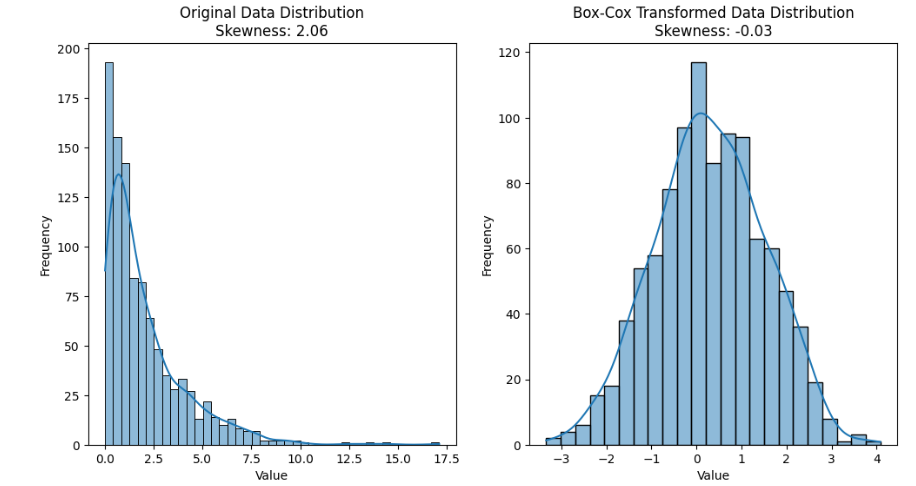
\includegraphics[width=0.75\linewidth]{imagenes/box-cox.png}
    \label{fig:box-cox}
\end{figure}

\subsection{Técnicas de discretización de datos}
Las técnicas de discretización convierten variables continuas en variables discretas, permitiendo ver los datos desde una perspectiva diferente. Este enfoque divide en rangos las variables continúas generando intervalos que tienen una etiqueta. De esta forma, el valor numérico pasa a una categoría o \textit{bins}.

Para el proceso de discretización, se pueden emplear árboles de decisión, para los que se aprovecha la \textbf{ganancia de información} como medida para delimitar los valores óptimos.

Otra técnica es el uso de cuantiles: dividir los valores continuos en cuatro cuantiles, donde cada cuantil encapsula una proporción igual de puntos de datos. 

\subsection{Técnicas de codificación de datos categóricos}
Los algoritmos de aprendizaje automático utilizan números y, por tanto, se hace necesario convertir los datos textuales a formato numérico.

La codificación es el proceso de convertir datos categóricos o textuales a numéricos, de modo que puedan usarse como entrada para que los procesen los algoritmos. Así, se permite que el modelo identifique patrones y haga predicciones basadas en esos patrones; esto ayuda a evitar sesgos al garantizar que todas las características tengan el mismo peso.

La elección del método de codificación puede tener un impacto significativo en el rendimiento del modelo, por lo que es importantes elegir una técnica adecuada según la naturaleza de los datos y los requisitos del modelo.

\begin{itemize}
    \item \textbf{Codificación One-Hot}: Una columna binaria se crea por cada categoría de la variable. Si la variable está presente se le asigna el valor de 1, si no se le asigna 0.

    \item \textbf{Codificación ordinal}: A cada categoría única se le asigna un valor entero único. Es más simple que la técnica anterior, pero tiene el inconveniente de que el algoritmo puede malinterpretar los números enteros asignados como si tuvieran una relación ordenada cuando no es el caso.

    \item \textbf{Codificación binaria}:  Las categorías se representan como dígitos binarios. Por ejemplo, si una variable tiene cuatro categorías  'Bueno',  'Malo',  'Regular'  y  'Excelente', se pueden representar como  0001, 0010, 0100 y 1000, respectivamente.

    \item \textbf{Codificación target}: Se utiliza con variables categóricas de alta cardinalidad; es decir, características con  muchas categorías únicas. Se calcula el valor objetivo promedio para cada categoría  y este valor promedio es utilizado para reemplazar la característica categórica.  Aunque toca utilizarla con precaución porque puede conducir a un sobreajuste.
\end{itemize}